\documentclass[aspectratio=169,10pt]{beamer}

\usepackage[T1]{fontenc}
\usepackage{lmodern}
\usepackage{graphicx}
\usepackage{booktabs}
\usepackage{array}
\usepackage{tikz}
\usepackage{xcolor}

\definecolor{Ink}{HTML}{20262B}
\definecolor{Navy}{HTML}{17324D}
\definecolor{Teal}{HTML}{168C88}
\definecolor{Amber}{HTML}{D99022}
\definecolor{Red}{HTML}{C94C4C}
\definecolor{Muted}{HTML}{697279}
\definecolor{Mist}{HTML}{E8EEF2}
\definecolor{Wash}{HTML}{F5F8FA}

\setbeamercolor{normal text}{fg=Ink,bg=white}
\setbeamercolor{frametitle}{fg=Navy,bg=white}
\setbeamerfont{frametitle}{size=\Large,series=\bfseries}
\setbeamertemplate{navigation symbols}{}
\setbeamersize{text margin left=.55cm,text margin right=.55cm}
\setbeamertemplate{frametitle}{%
  \vspace{.18cm}\insertframetitle\par\vspace{-.10cm}%
  \color{Teal}\rule{1.0cm}{1.4pt}\color{Mist}\rule{\dimexpr\textwidth-1.0cm\relax}{1.4pt}}
\setbeamertemplate{footline}{%
  \leavevmode\hbox{\begin{beamercolorbox}[wd=.82\paperwidth,ht=2.6ex,dp=1ex,leftskip=.55cm]{normal text}%
  \color{Muted}\scriptsize FOR2107 resting-state comparison · preliminary · 1 September 2026
  \end{beamercolorbox}\begin{beamercolorbox}[wd=.18\paperwidth,ht=2.6ex,dp=1ex,rightskip=.55cm plus1fil]{normal text}%
  \color{Muted}\scriptsize\insertframenumber/5
  \end{beamercolorbox}}}

\newcommand{\sourceNote}[1]{\vspace{.04cm}{\color{Muted}\tiny #1}}
\newcommand{\paneltitle}[1]{{\color{Navy}\bfseries\small #1}}

\begin{document}

\begin{frame}[plain]
  \vfill
  
\begin{tikzpicture}
    \fill[Teal] (0,0) rectangle (1.1,.10);
    \fill[Navy] (1.25,0) rectangle (5.2,.10);
  \end{tikzpicture}
  \vspace{.30cm}

  {\color{Navy}\fontsize{28}{32}\selectfont\bfseries Visual cross-check of resting-state clustering\par}
  \vspace{.18cm}
  {\color{Muted}\Large FOR2107 compared with Tozzi et al.\par}
  \vspace{.48cm}
  \vfill
  {\color{Muted}\small Preliminary comparison · five- and six-cluster descriptive solutions · 1 September 2026}
\end{frame}

\begin{frame}{FOR2107 data sample}
\centering
\begin{beamercolorbox}[rounded=true,sep=.16cm,wd=.96\textwidth]{normal text}
  \centering\color{Navy}\normalsize\textbf{2,239 participants in the selected FOR2107 cohort}
\end{beamercolorbox}
\vspace{.38cm}
\begin{columns}[T,onlytextwidth]
  \begin{column}{.47\textwidth}
    \begin{beamercolorbox}[rounded=true,sep=.18cm,wd=\linewidth]{normal text}
      \centering{\color{Teal}\fontsize{25}{27}\selectfont\bfseries 1,130}\par
      \vspace{.03cm}{\color{Navy}\bfseries Healthy reference participants}
    \end{beamercolorbox}
  \end{column}
  \begin{column}{.47\textwidth}
    \begin{beamercolorbox}[rounded=true,sep=.18cm,wd=\linewidth]{normal text}
      \centering{\color{Amber}\fontsize{25}{27}\selectfont\bfseries 1,109}\par
      \vspace{.03cm}{\color{Navy}\bfseries Clinical participants}
    \end{beamercolorbox}
  \end{column}
\end{columns}
\vspace{.18cm}
\renewcommand{\arraystretch}{1.32}
\setlength{\tabcolsep}{8pt}
\begin{tabular}{>{\raggedright\arraybackslash}m{5.35cm} >{\centering\arraybackslash}m{2.05cm} >{\raggedright\arraybackslash}m{4.95cm}}
  \toprule
  \textbf{Clinical diagnosis} & \textbf{n} & \textbf{Role in current analysis} \\
  \midrule
  MDD & 823 & Primary clinical group \\
  Anxiety + comorbid MDD & 266 & Included with clinical group \\
  Anxiety-only & 20 & Included with clinical group \\
  \midrule
  \textbf{Total clinical} & \textbf{1,109} & MDD + anxiety analysis \\
  \bottomrule
\end{tabular}
\vspace{0cm}
\centering\color{Muted}\scriptsize Clustering input: 2,237 participants (1,108 clinical; 1,129 healthy reference).
\end{frame}

\begin{frame}{Supplementary Figure 2: how convincing is the separation?}
\centering
\begin{columns}[T,onlytextwidth]
  \begin{column}{.325\textwidth}
    \centering\paneltitle{Tozzi et al.}\par\vspace{.08cm}
    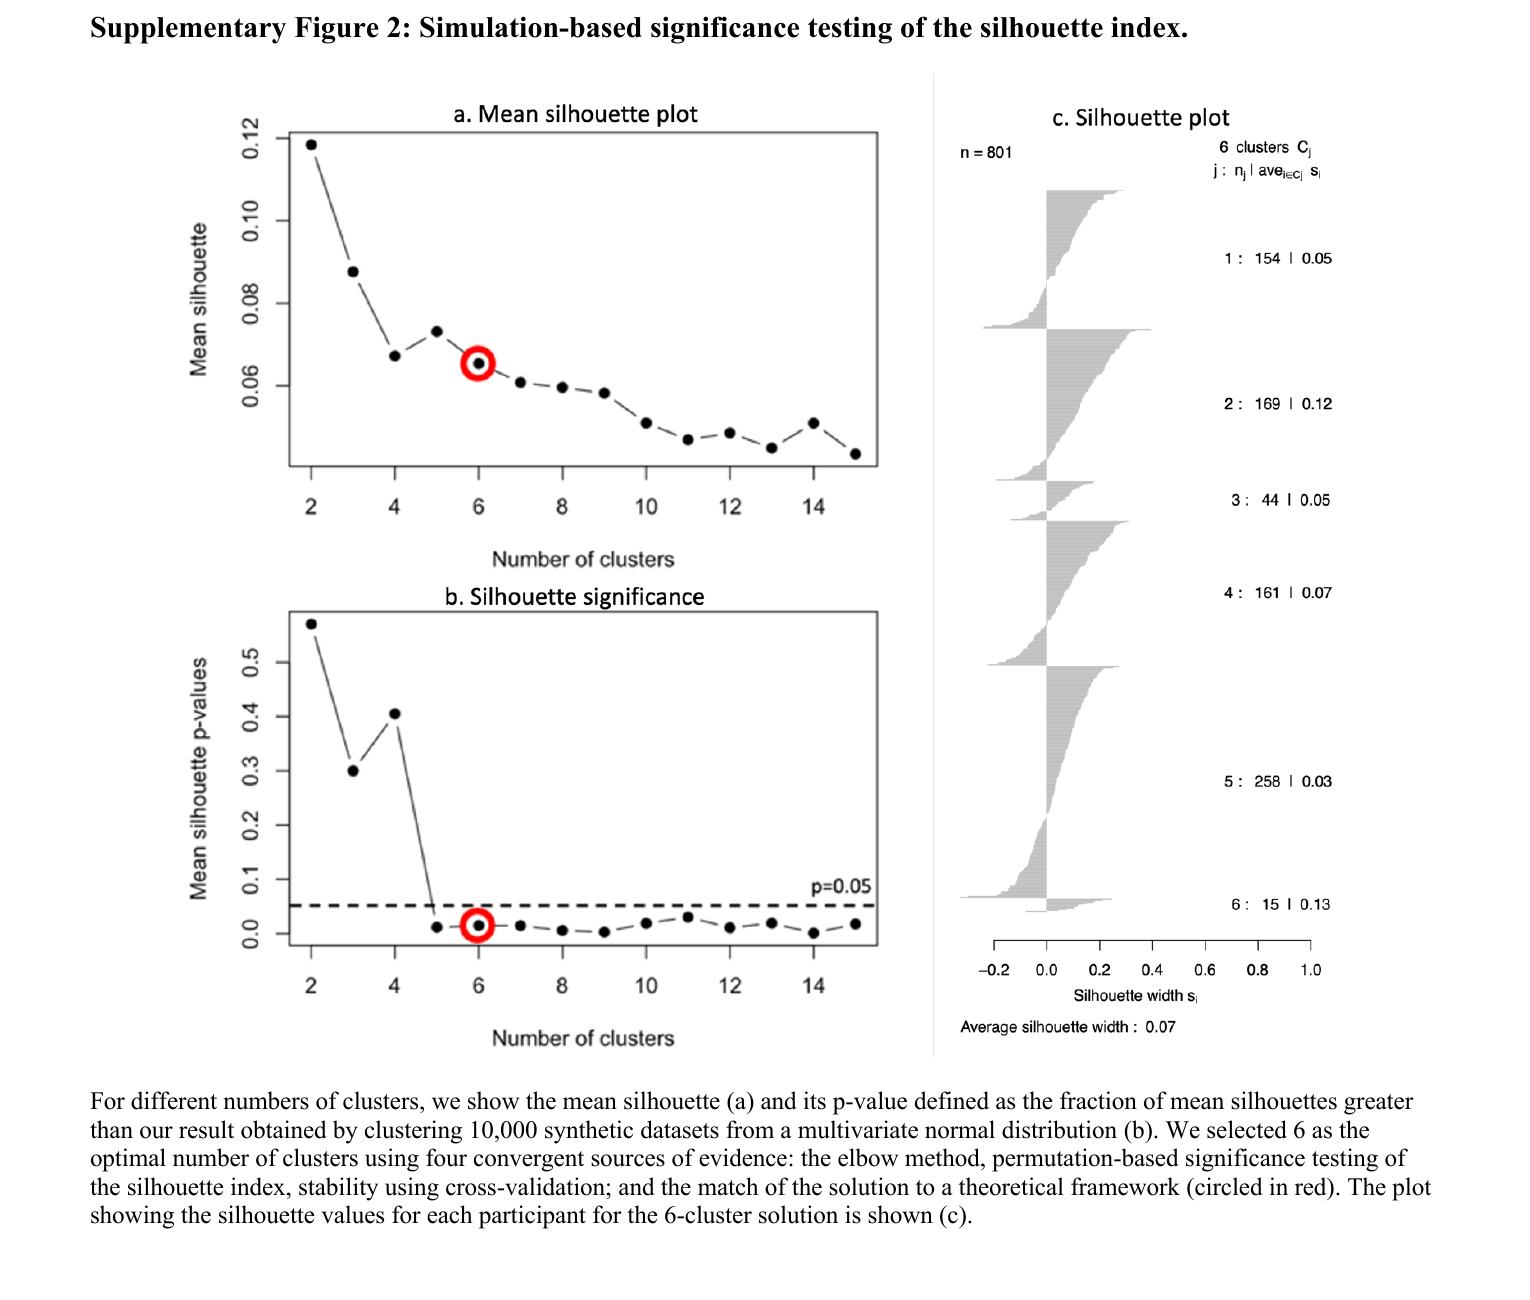
\includegraphics[width=\linewidth,height=.68\textheight,keepaspectratio]{figures/tozzi_supp_fig2.png}\par
  \end{column}
  \begin{column}{.325\textwidth}
    \centering\paneltitle{FOR2107 · k = 6}\par\vspace{.08cm}
    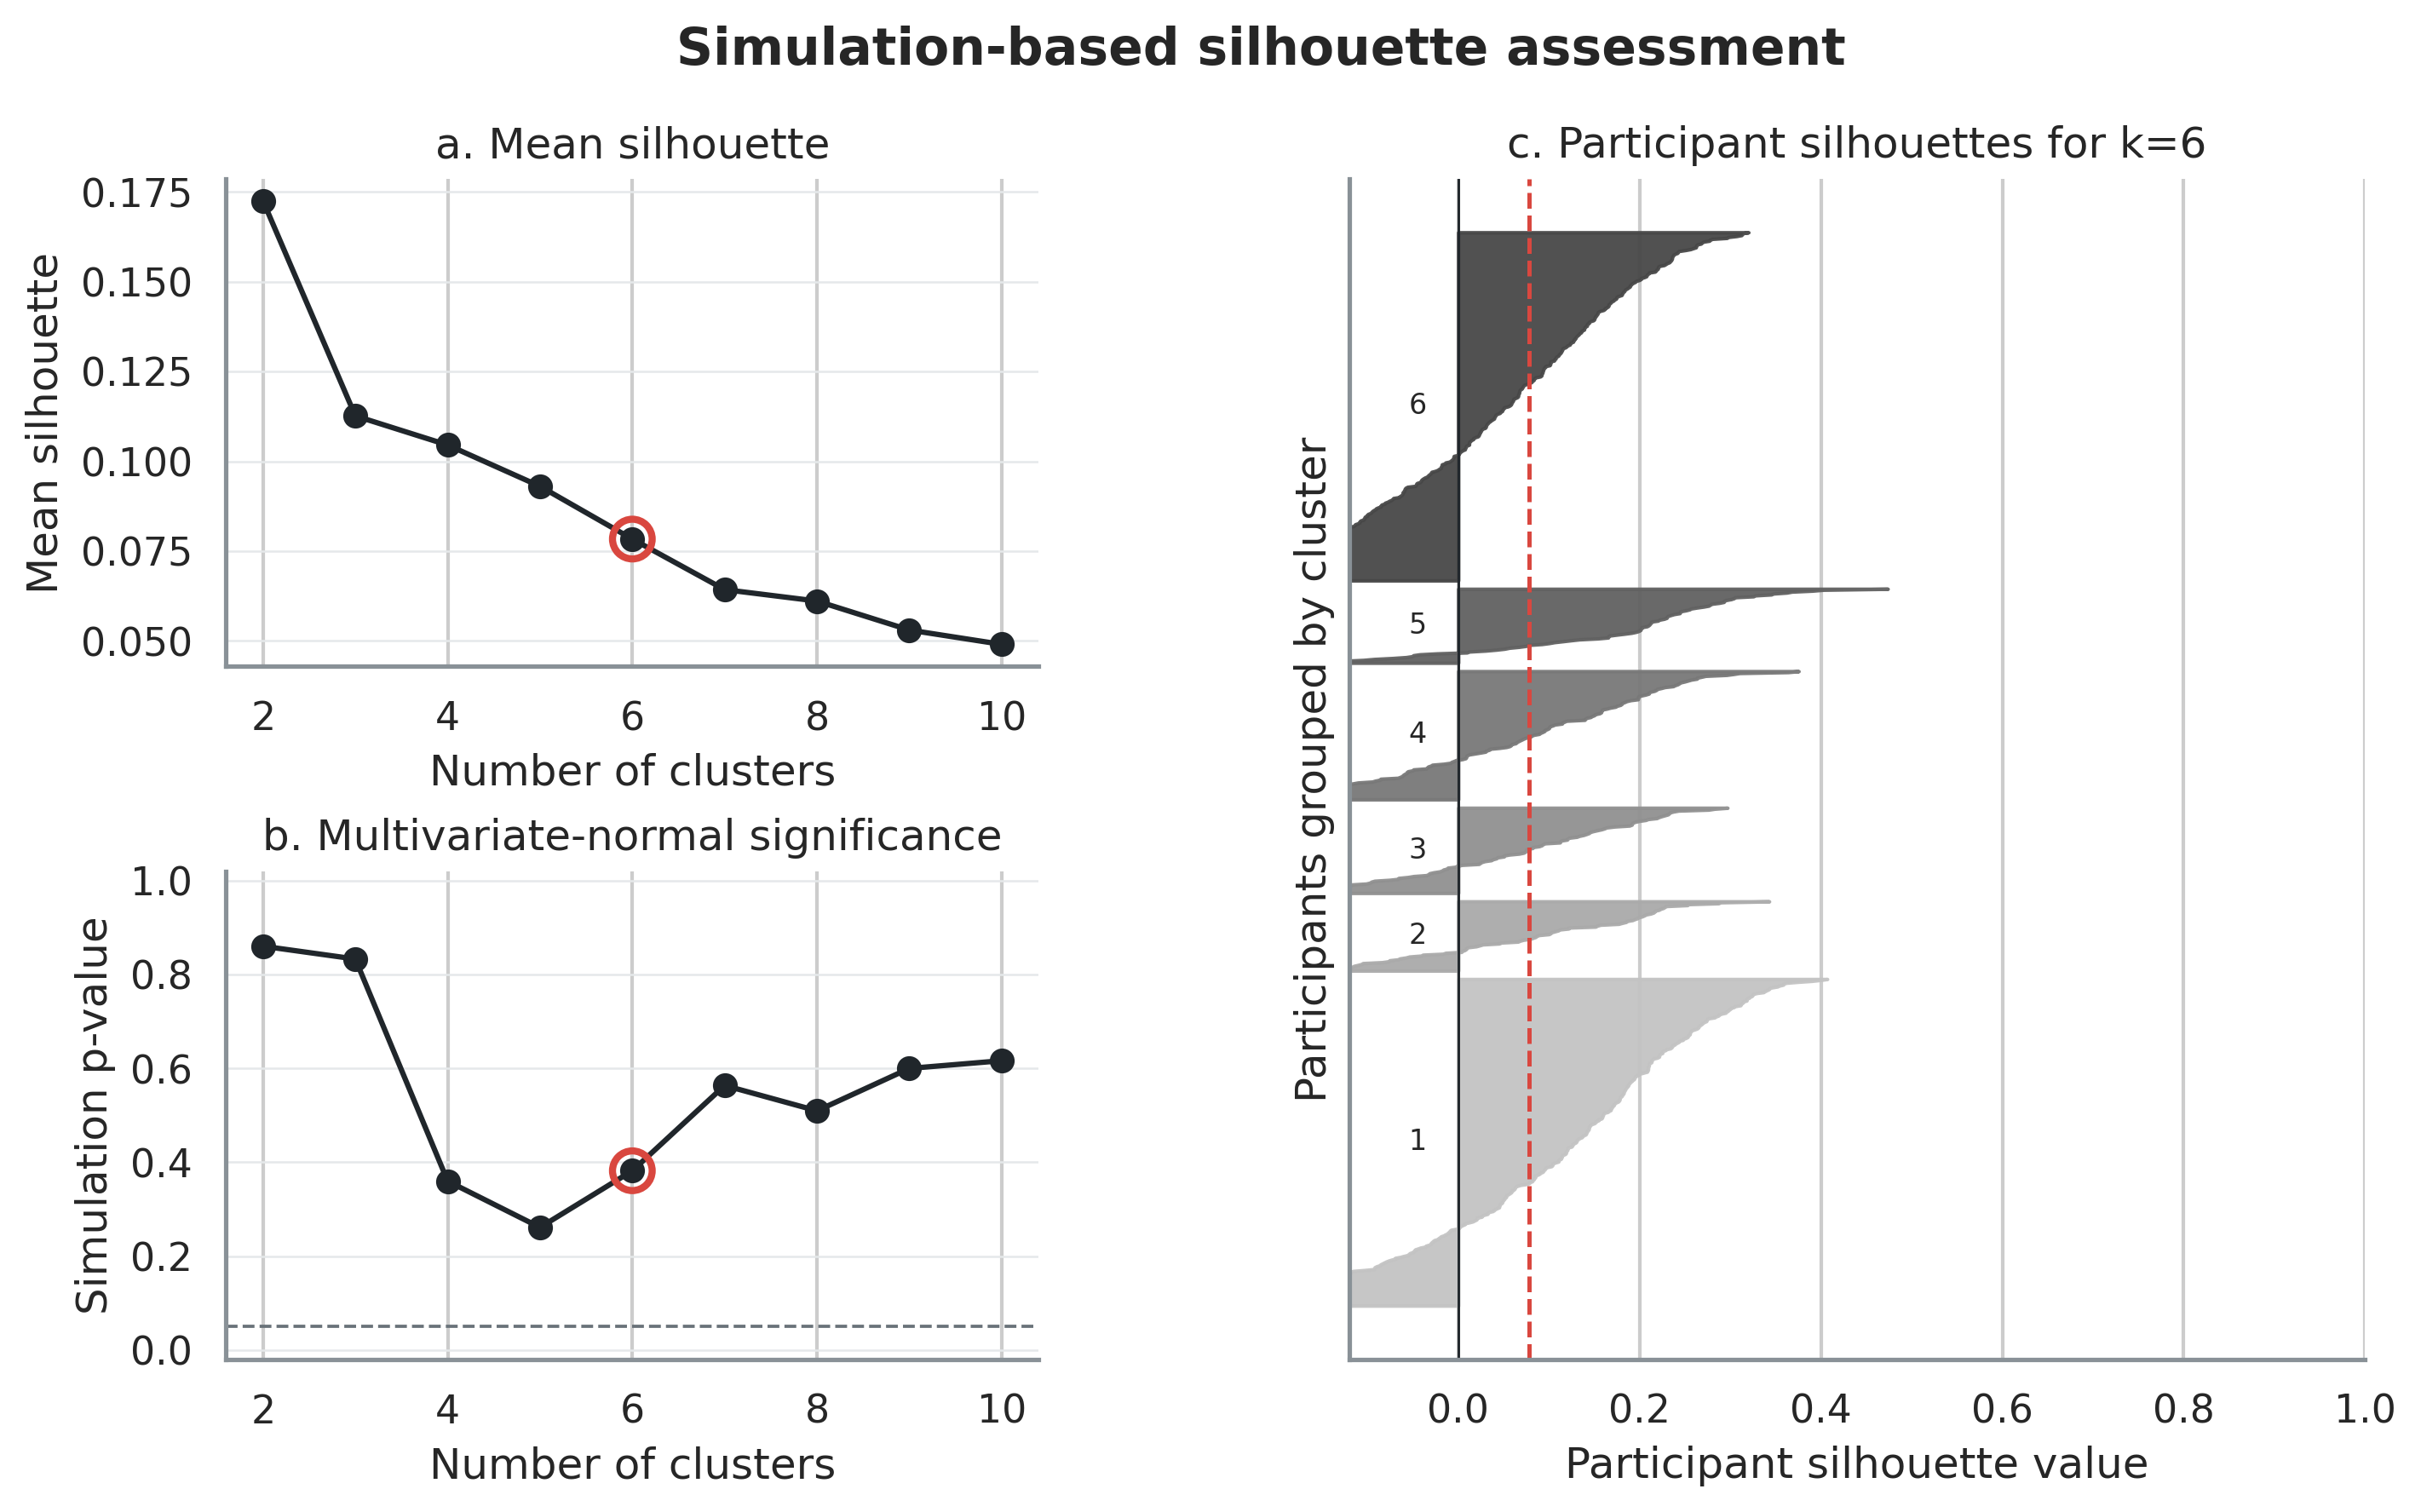
\includegraphics[width=\linewidth,height=.68\textheight,keepaspectratio]{figures/supplementary_figure_2_k6.png}\par
  \end{column}
  \begin{column}{.325\textwidth}
    \centering\paneltitle{FOR2107 · k = 5}\par\vspace{.08cm}
    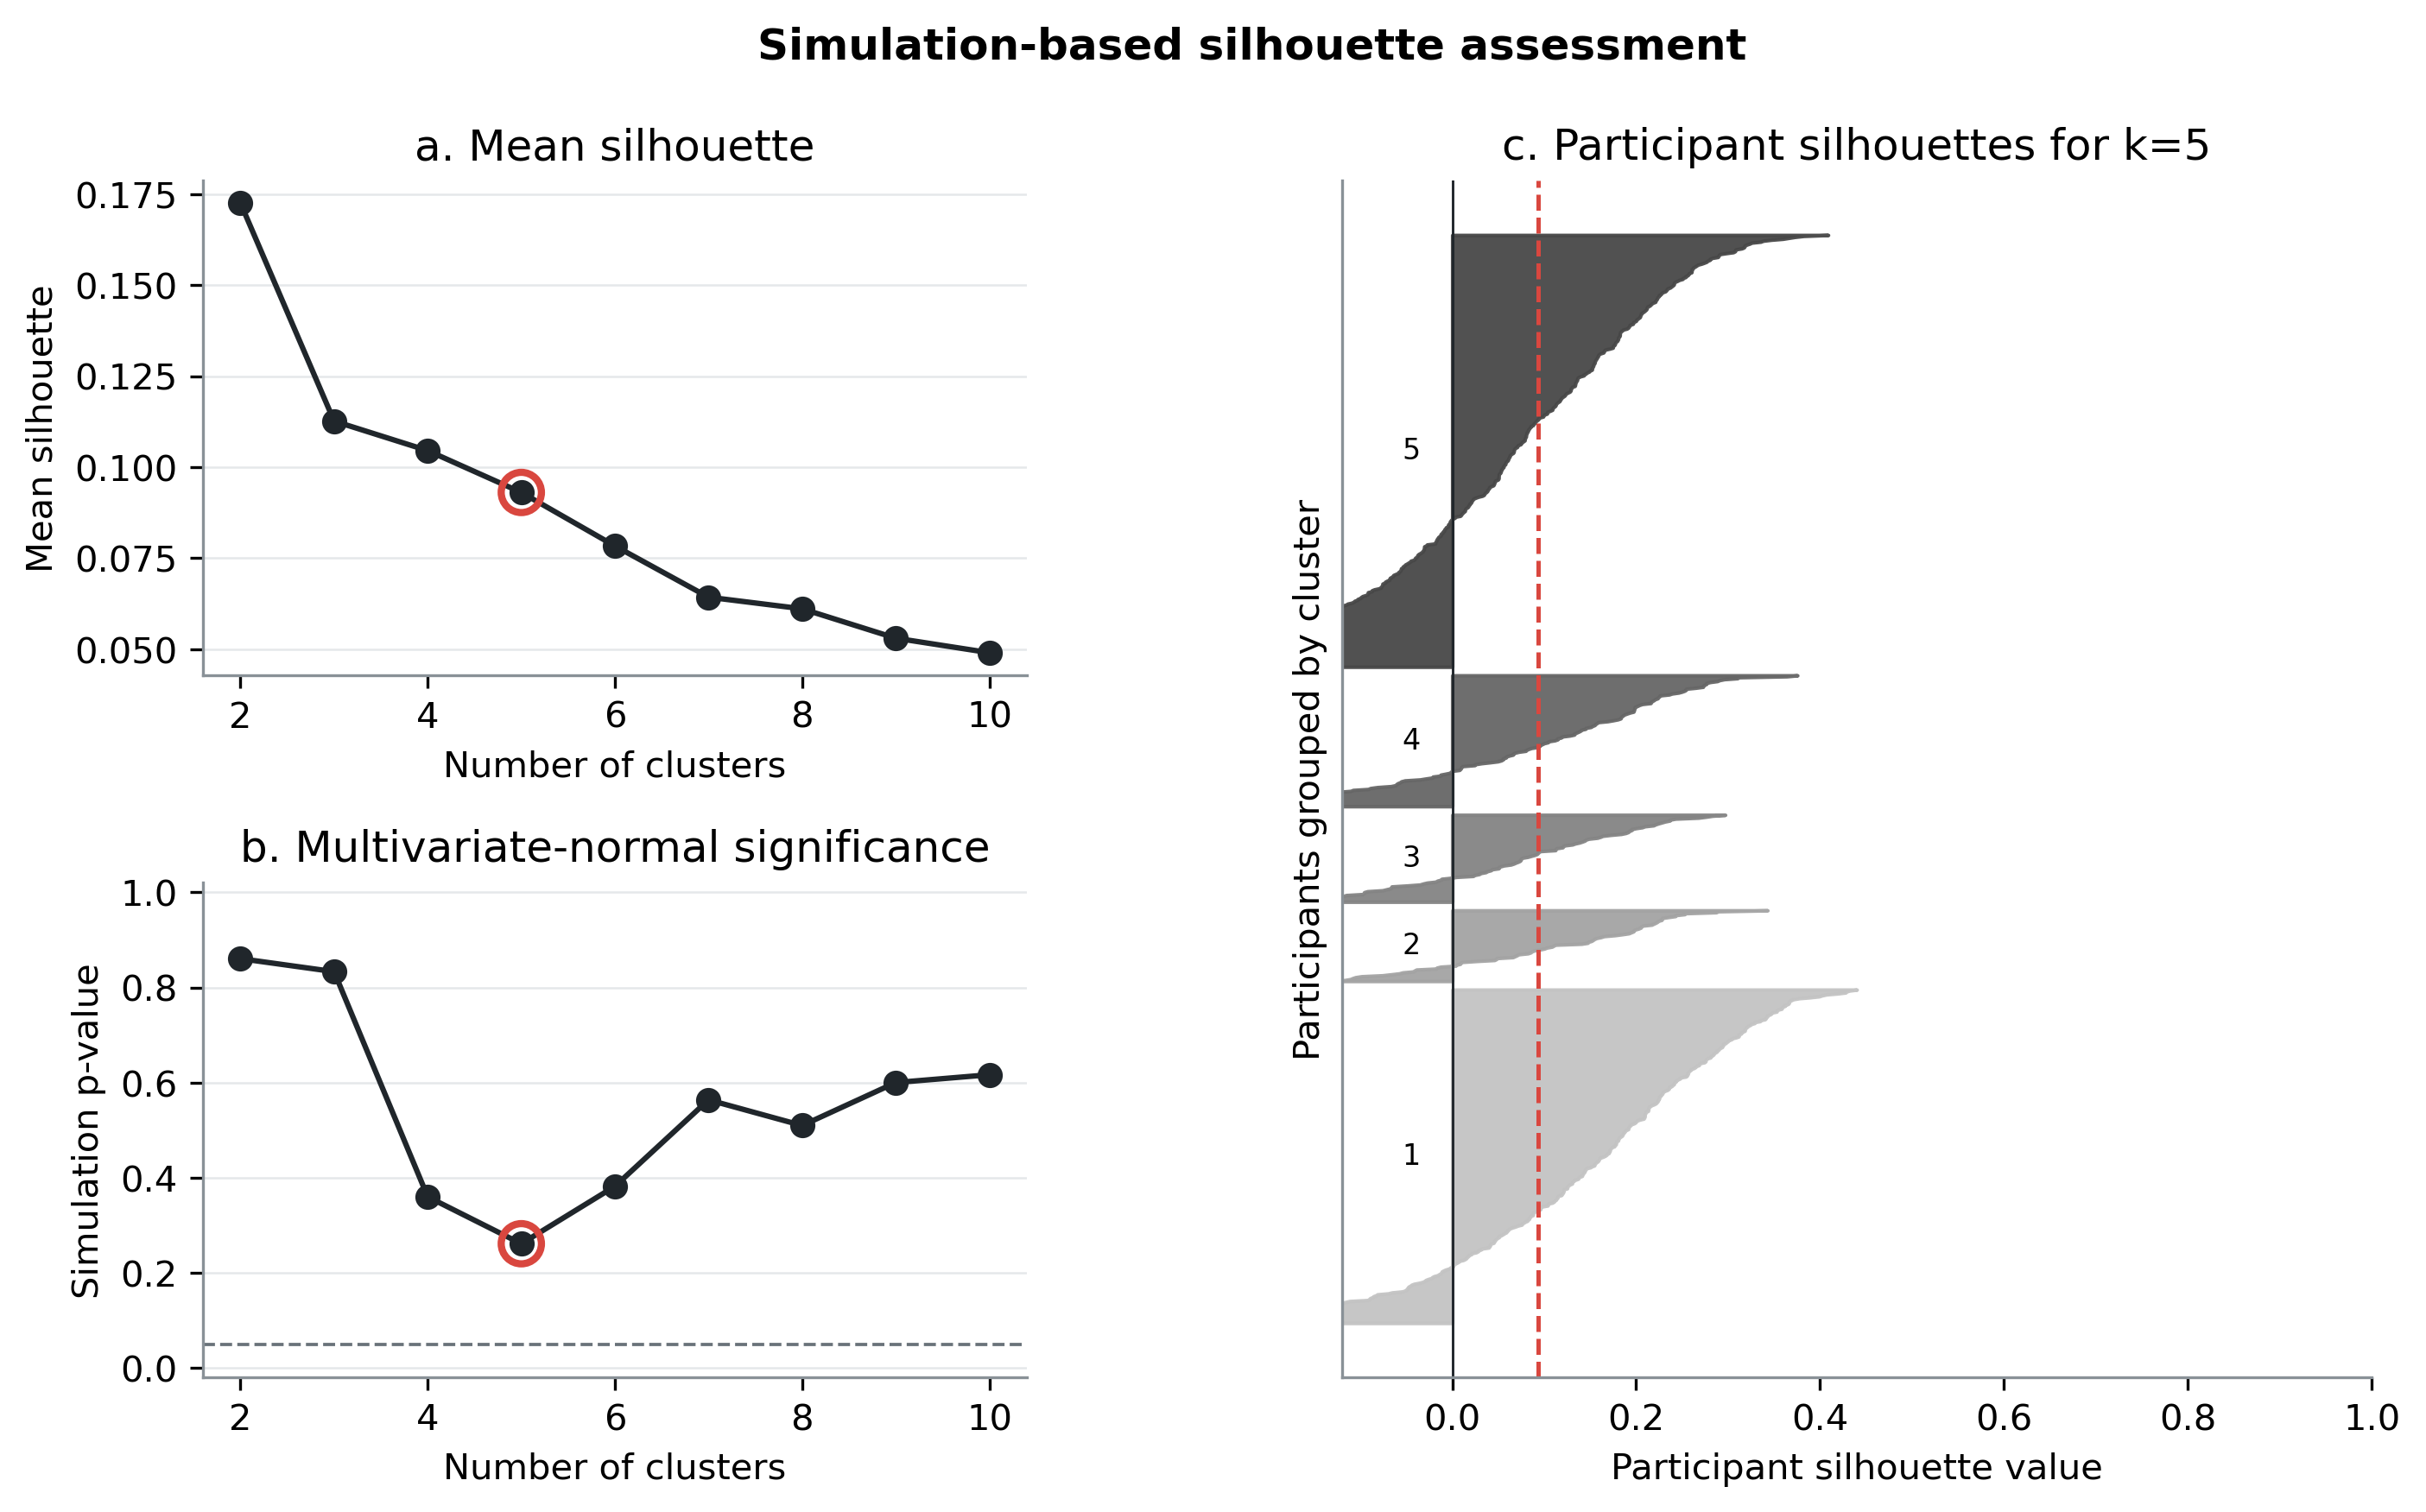
\includegraphics[width=\linewidth,height=.68\textheight,keepaspectratio]{figures/supplementary_figure_2_k5.png}\par
  \end{column}
\end{columns}
\end{frame}

\begin{frame}{Supplementary Figure 5: what do the cluster profiles look like?}
\centering
\begin{columns}[T,onlytextwidth]
  \begin{column}{.325\textwidth}
    \centering\paneltitle{Tozzi et al.}\par\vspace{.06cm}
    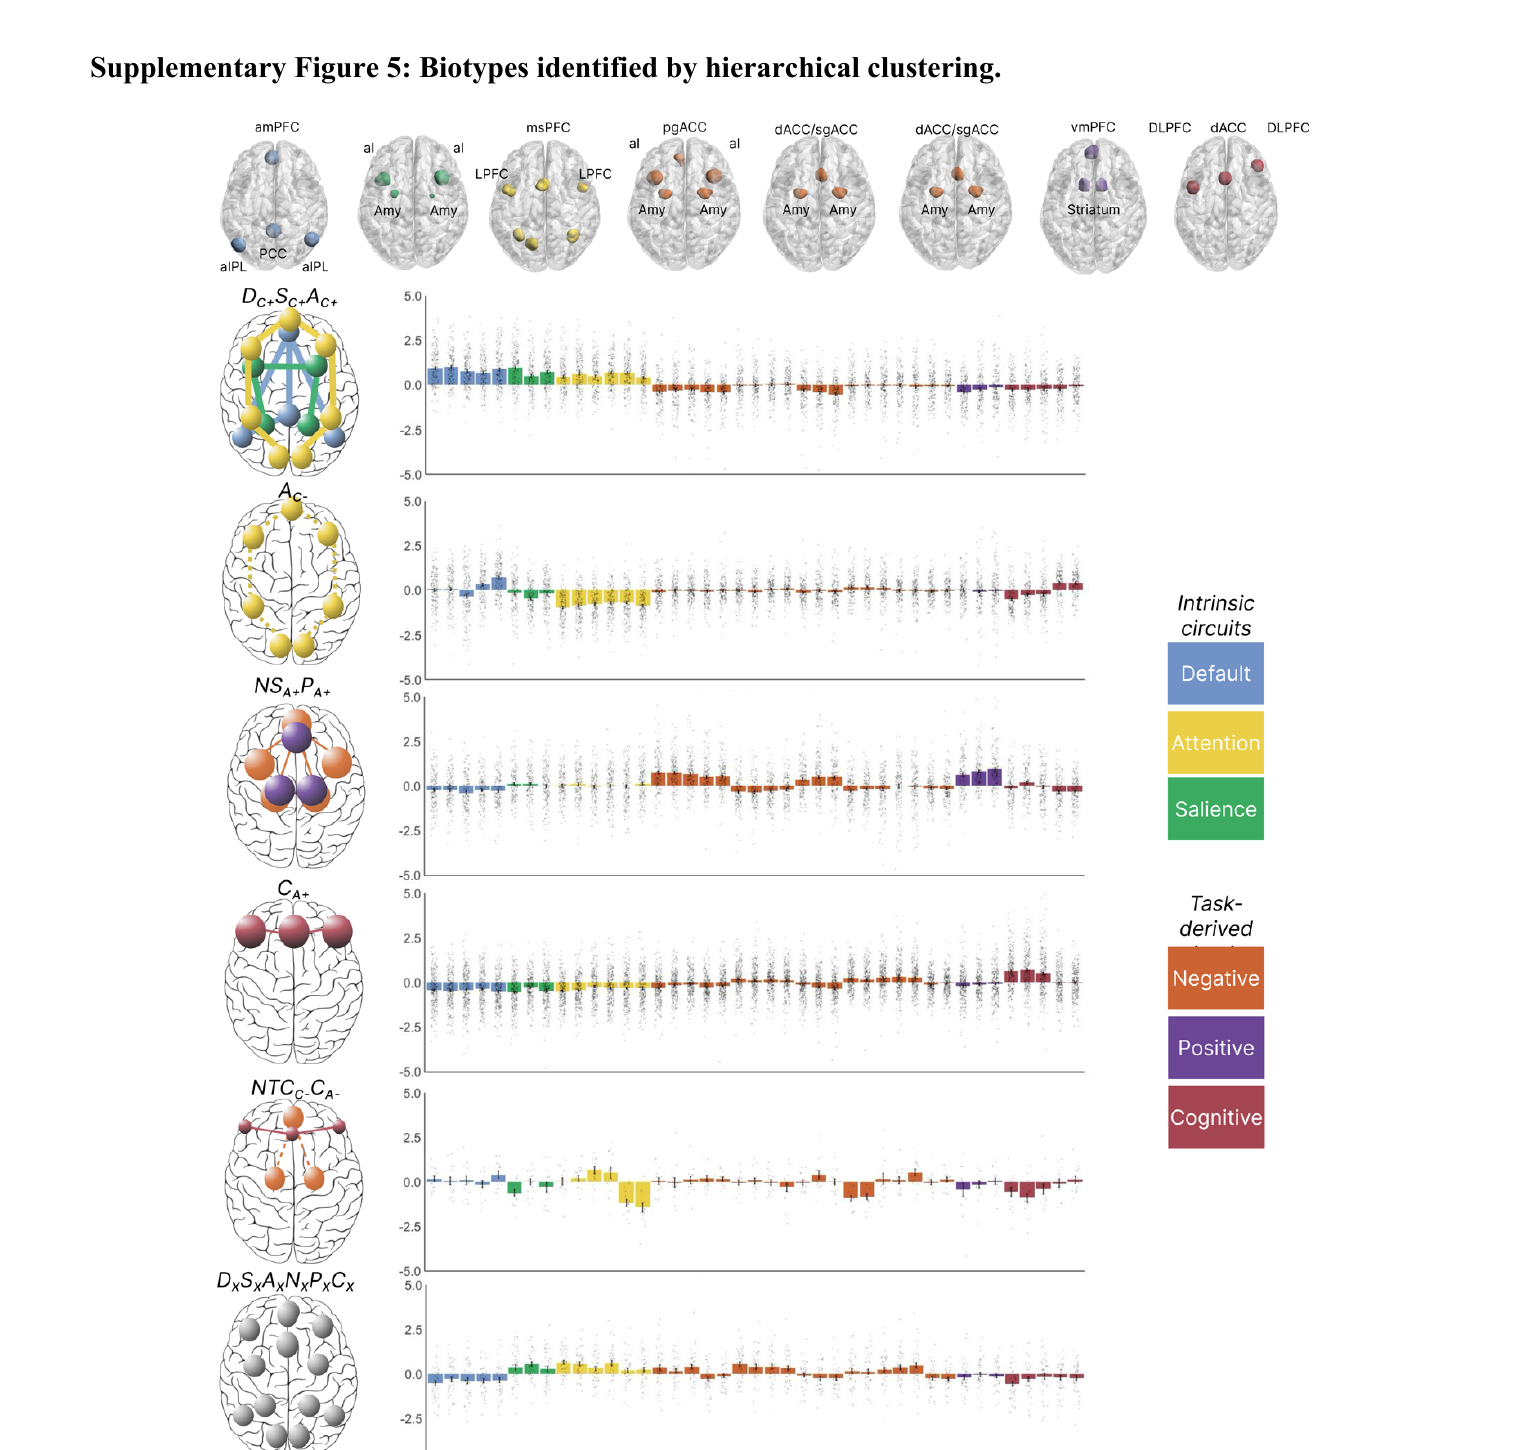
\includegraphics[width=\linewidth,height=.75\textheight,keepaspectratio]{figures/tozzi_supp_fig5.png}\par
  \end{column}
  \begin{column}{.325\textwidth}
    \centering\paneltitle{FOR2107 · k = 6}\par\vspace{.06cm}
    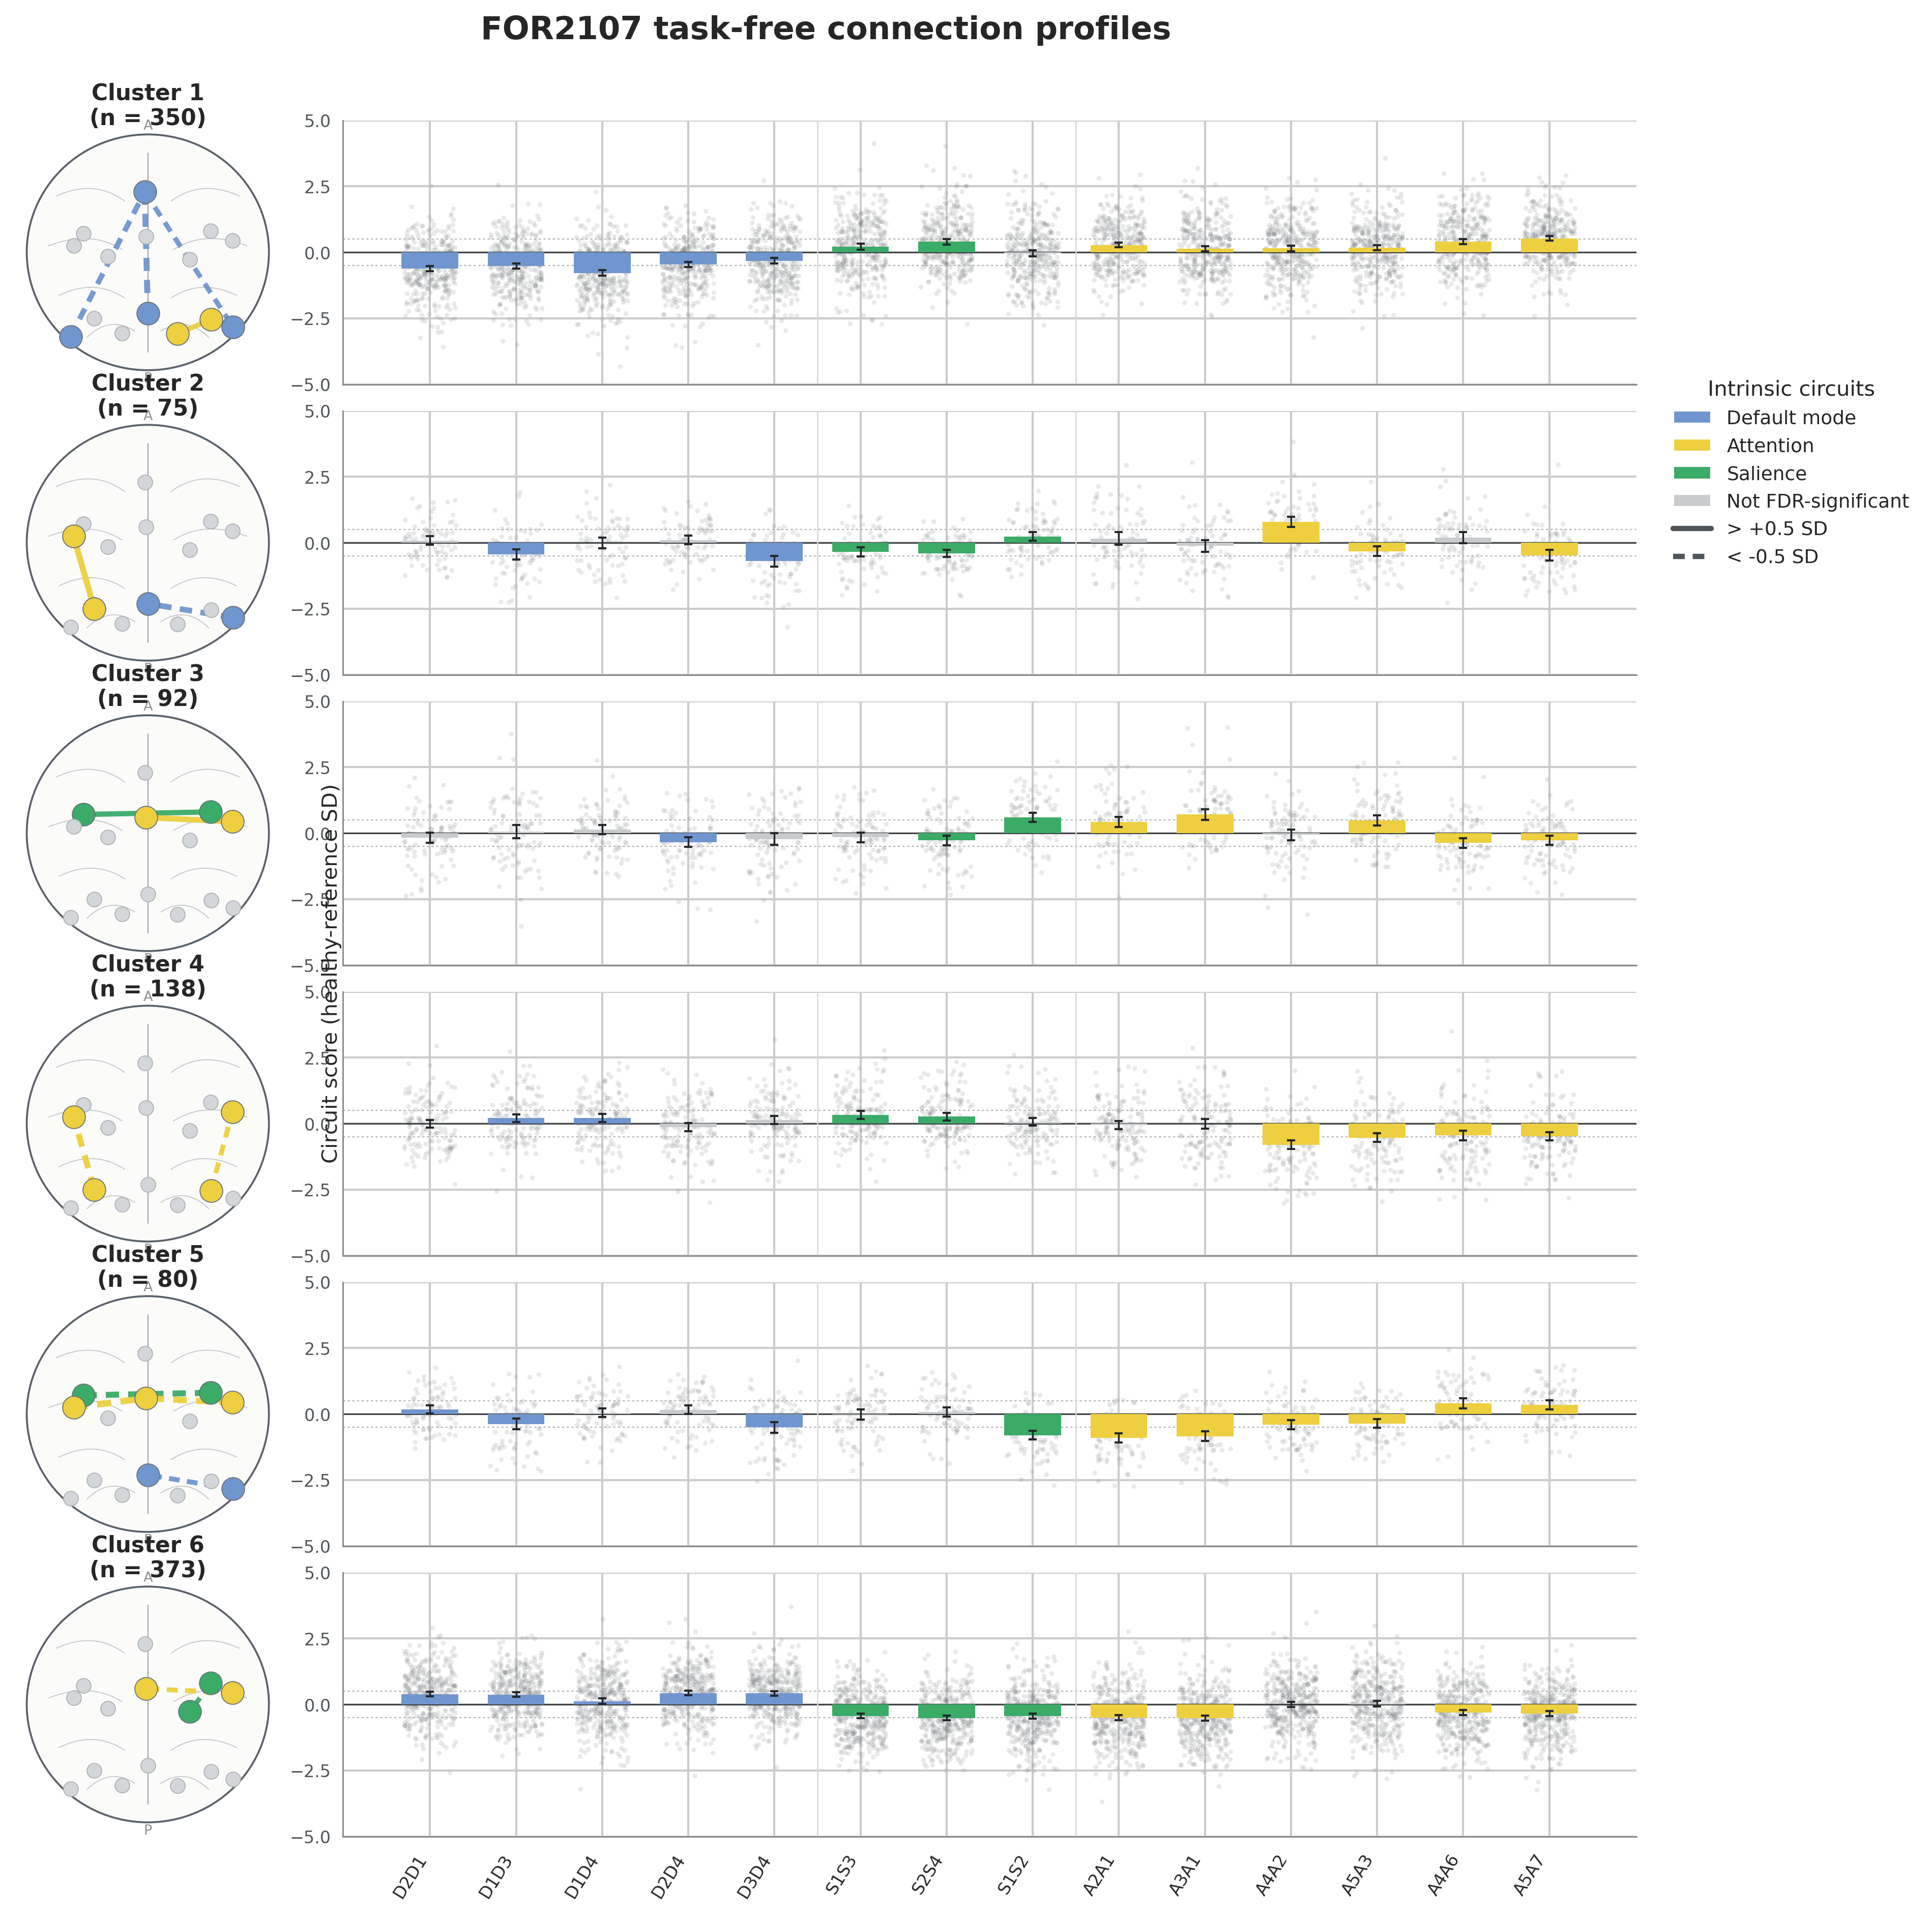
\includegraphics[width=\linewidth,height=.75\textheight,keepaspectratio]{figures/tozzi_style_k6.png}\par
  \end{column}
  \begin{column}{.325\textwidth}
    \centering\paneltitle{FOR2107 · k = 5}\par\vspace{.06cm}
    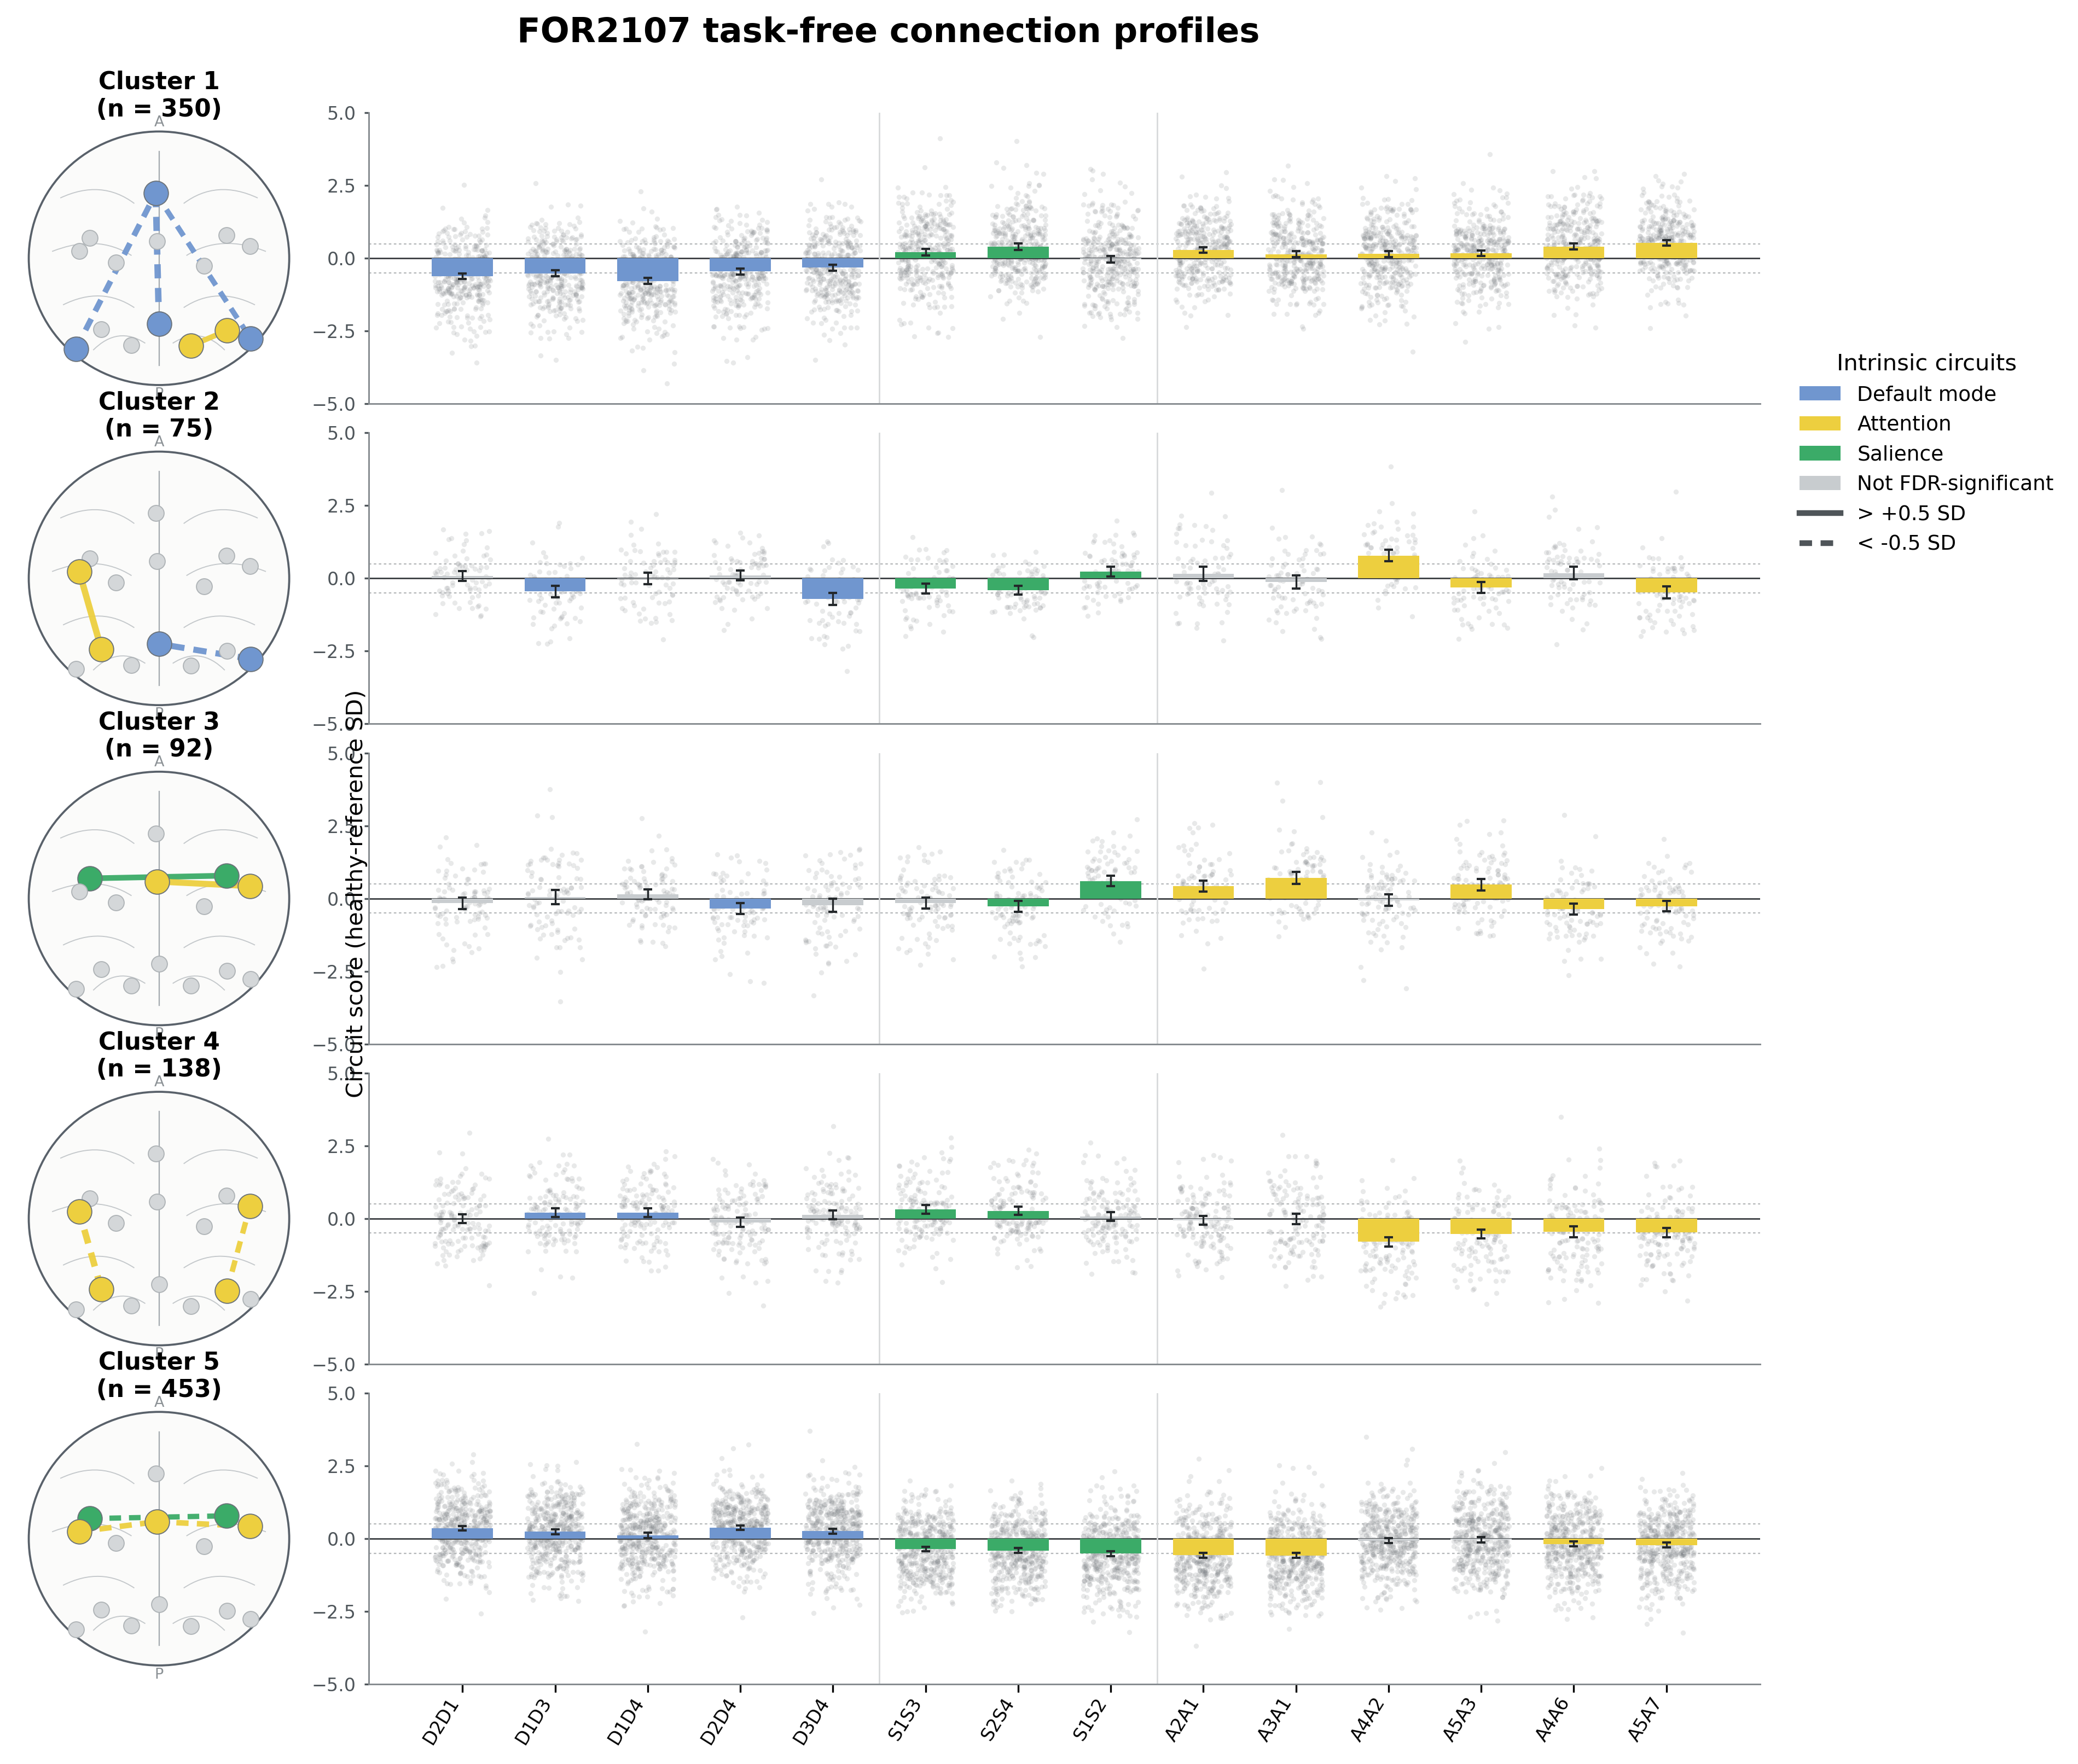
\includegraphics[width=\linewidth,height=.75\textheight,keepaspectratio]{figures/tozzi_style_k5.png}\par
  \end{column}
\end{columns}
\end{frame}

\begin{frame}{Task equivalence and the replication boundary}
\small
\renewcommand{\arraystretch}{1.32}
\setlength{\tabcolsep}{4pt}
\centering
\begin{tabular}{>{\raggedright\arraybackslash}m{5.55cm} >{\centering\arraybackslash\bfseries}m{1.55cm} >{\raggedright\arraybackslash}m{5.85cm}}
  \toprule
  \multicolumn{1}{c}{\textbf{Tozzi et al.}} &
  \multicolumn{1}{c}{\textbf{Relationship}} &
  \multicolumn{1}{c}{\textbf{FOR2107}} \\
  \midrule
  Task-free fMRI scan & \color{Teal}Close & Resting-state fMRI scan \\
  Conscious Facial Expressions of Emotion Task & \color{Amber}Related & Face-matching task \\
  Non-conscious Facial Expressions of Emotion Task & \color{Amber}Related & Subliminal affective-priming task \\
  Go--NoGo Task & \color{Red}Missing & No direct equivalent \\
  No equivalent & \color{Navy}Additional & Episodic memory-encoding task \\
  \bottomrule
\end{tabular}

\vfill
\begin{beamercolorbox}[rounded=true,sep=.22cm,wd=.96\textwidth]{normal text}
  \centering\color{Navy}\normalsize\bfseries Without the exact data acquisition protocol, we doubt that the results can be reproduced exactly.
\end{beamercolorbox}
\end{frame}

\end{document}
